% Options for packages loaded elsewhere
\PassOptionsToPackage{unicode}{hyperref}
\PassOptionsToPackage{hyphens}{url}
%
\documentclass[
]{article}
\usepackage{amsmath,amssymb}
\usepackage{lmodern}
\usepackage{ifxetex,ifluatex}
\ifnum 0\ifxetex 1\fi\ifluatex 1\fi=0 % if pdftex
  \usepackage[T1]{fontenc}
  \usepackage[utf8]{inputenc}
  \usepackage{textcomp} % provide euro and other symbols
\else % if luatex or xetex
  \usepackage{unicode-math}
  \defaultfontfeatures{Scale=MatchLowercase}
  \defaultfontfeatures[\rmfamily]{Ligatures=TeX,Scale=1}
\fi
% Use upquote if available, for straight quotes in verbatim environments
\IfFileExists{upquote.sty}{\usepackage{upquote}}{}
\IfFileExists{microtype.sty}{% use microtype if available
  \usepackage[]{microtype}
  \UseMicrotypeSet[protrusion]{basicmath} % disable protrusion for tt fonts
}{}
\makeatletter
\@ifundefined{KOMAClassName}{% if non-KOMA class
  \IfFileExists{parskip.sty}{%
    \usepackage{parskip}
  }{% else
    \setlength{\parindent}{0pt}
    \setlength{\parskip}{6pt plus 2pt minus 1pt}}
}{% if KOMA class
  \KOMAoptions{parskip=half}}
\makeatother
\usepackage{xcolor}
\IfFileExists{xurl.sty}{\usepackage{xurl}}{} % add URL line breaks if available
\IfFileExists{bookmark.sty}{\usepackage{bookmark}}{\usepackage{hyperref}}
\hypersetup{
  hidelinks,
  pdfcreator={LaTeX via pandoc}}
\urlstyle{same} % disable monospaced font for URLs
\usepackage[margin=1in]{geometry}
\usepackage{longtable,booktabs,array}
\usepackage{calc} % for calculating minipage widths
% Correct order of tables after \paragraph or \subparagraph
\usepackage{etoolbox}
\makeatletter
\patchcmd\longtable{\par}{\if@noskipsec\mbox{}\fi\par}{}{}
\makeatother
% Allow footnotes in longtable head/foot
\IfFileExists{footnotehyper.sty}{\usepackage{footnotehyper}}{\usepackage{footnote}}
\makesavenoteenv{longtable}
\usepackage{graphicx}
\makeatletter
\def\maxwidth{\ifdim\Gin@nat@width>\linewidth\linewidth\else\Gin@nat@width\fi}
\def\maxheight{\ifdim\Gin@nat@height>\textheight\textheight\else\Gin@nat@height\fi}
\makeatother
% Scale images if necessary, so that they will not overflow the page
% margins by default, and it is still possible to overwrite the defaults
% using explicit options in \includegraphics[width, height, ...]{}
\setkeys{Gin}{width=\maxwidth,height=\maxheight,keepaspectratio}
% Set default figure placement to htbp
\makeatletter
\def\fps@figure{htbp}
\makeatother
\setlength{\emergencystretch}{3em} % prevent overfull lines
\providecommand{\tightlist}{%
  \setlength{\itemsep}{0pt}\setlength{\parskip}{0pt}}
\setcounter{secnumdepth}{-\maxdimen} % remove section numbering
\ifluatex
  \usepackage{selnolig}  % disable illegal ligatures
\fi

\author{}
\date{\vspace{-2.5em}}

\begin{document}

\section{Rheological Profile of structure formation in model processed cheese}
\subsection{Introduction}

The rheological profile or generally spoken the viscosity of dispersed
systems in the food, pharmaceutical or cosmetic industry is an important
parameter for the quality assurance of such products. Additionally, the
rheological behaviour under certain process conditions can give insight
towards the structuring mechanisms occuring on a molecular level. Many
studies have been performed on dispersed an highly concentrated food
systems such as processed cheese. Most of them were compositional in
nature (see also Tablexx in section 1), meaning that effects of certain
educt components on the properties of the final product were
investigated. @Salek2017 investigated the effects of special mixtures of
emulsifying salts on the hardness of processed cheeses. Maximum hardness
was achieved by a combination of DSP and TSPP. @Cunha2013 studied the
effects of different types of fat (hardened and non hardened plant oil
in comparison to butter) on the texture of processed cheese. Samples
made with both plant oils showed lower fat globule size, higher
viscosity and higher hardness than those made with butter.

The step-wise structure build-up has been described in detail by
@Lenze2019. The aggregation process was identified as the formation of a
continously aggregated protein matrix wherein the fat is first
emulsified and then de-emulsified prior to network formation of the
proteins. To the authors knowledge, either other proteinogenic entities
than predominantly casein were present during processing, or surface
active ingredients or dairy cream was used as the fat phase, hence the
structuring and simultaneous emulsifying properties of casein alone has
not yet been determined. The TEM images obtained by @Vollmer2021 are
from samples that were free of proteins or surfactants other than
casein. The samples were prepared by the author, with reduced processing
speed in order to get a detailed representation of the structure
formation processes occuring. TEM imaging revealed the early presence of
fibrillar structures, that hold the fat in the matrix and also form a
dense network.

Step-wise structure formations were also detected in the works of
@Noronha2008 and @Noronha2008c. Two peaks were detectable during
processing of a modell processed cheese in a blade cooker. The first
peak or increase was attributed to water uptake and the formation of a
hydrated casein matrix, since it was reported that ∼75\% of the added
water was absorbed. Subsequently, a fat emulsification took place. After
sufficient emulsification of the dispersed phase, the fat particles were
reported to be incorporated into the cheese matrix which lead to the
formation of a cohesive matrix as indicated by a second peak.

It has already been shown by others that initially micellar casein
sources such as native casein or rennet casein only perform the process
known as ``creaming reaction'' under the presence of emulsifying salts.
The micelle must be (at least partially) dissociatied to form new
structures. When using sodium caseinate as source material, no such
dissociation is necessary or even possible, since the caseins are
already present in monomeric form. In order to get an overview of the
structure formation induced by casein overall, several model cheeses
with varying protein sources are produced in this study: rennet casein,
native casein and sodium caseinate. Salt composition is varied in
samples made from sodium caseinate using HCl and citric acid in order to
investigate potential structure formation processes that occur from
caseins alone without the addition of melting salts. A further
simplified model system was used, which contained 15\% total protein for
the structure formation and 20\% fat (plant oil). The dry matter of the
system is around 40\%. In order to investigate structural changes during
processing, the dairy matrix can be processed in a shear-stress
rheometer, in which the structure build-up under controlled shear and
heat can be followed as in @Lenze2019.

The aim was to find two distinctly different rheological profiles in
order to further investigate (chapter 4) if the changes in rheological
behaviour can also be seen in distributional and compositional data of
the matrix, analyzed at multiple steps of processing.

\subsection{Material and Methods}

\textbf{Production of model process cheese premix} \newline The
composition of the processed cheese premix used corresponded to the
model processed cheese recipe developed by @Lenze2019 as follows:

\begin{longtable}[]{@{}lll@{}}
\caption{Recipe for the model processed cheese investigated throughout
this study}\tabularnewline
\toprule
Ingredient & Source & Amount (w/w, \%) \\
\midrule
\endfirsthead
\toprule
Ingredient & Source & Amount (w/w, \%) \\
\midrule
\endhead
Protein & Casein (rennet, native or sodium) & 18.42 \\
Fat & Sunflower oil & 19.59 \\
Water & Milli-Q water & 58.48 \\
Emulsifying salt & Trisodium citrate, dibasic (Na3C6H5O7·H2O) & 0.44 \\
--- & Disodium phosphate dihydrate (Na2HPO4·2H2O) & 0.44 \\
--- & Pentasodium triphosphate (Na5P3O10) & 1.75 \\
Acid for target pH=5.88 & Citric acid monohydrate (C6H8O7·H2O) & 0.88 \\
\bottomrule
\end{longtable}

The emulsifying salts displayed in Tablexx stayed the same throughout
this trial to ensure an equal dissociation of the caseins and therefore
making the single analyses compareable with each other. In the
subsequent sections of this work, the single emulsifying salts will be
referred to as their abbreviations (i.e.~TSC, DSP, PP) shown in Tablexx.
Also when speaking of ``the emulsifying salts'' or ``the emulsifying
salt mixture'' or ``the melting salts'', the combination of these salts
with citric acid as acidulent is meant. In Figures and plots within this
work, the term ``emS'' is used as abbreviation for the emulsifying or
melting salt combination.

The recipe displayed in Tablexx is based on the original product; yet,
influencing factors such as the type of fat or the age of the cheese can
be reduced in order to obtain a system that is as reproducible and
comparable as possible. In the course of the present work, native
(micellar) casein, rennet casein and sodium caseinate were used as
protein sources. Sodium and rennet casein were commercially available
products (ICL, Tel Aviv, Israel), the native casein was produced as it
was described in detail in @Dumpler2018. Sunflower oil was used as fat.
The pH value, which should be \textasciitilde5.88, was adjusted using
powdered citric acid. The melting salts were also weighed out as powder
the dry matter.

The individual recipe components were weighed into a beaker on an
analytical balance. The protein powder was weighed separately into a
weighing dish. The protein-oil-water dispersion was prepared with the
aid of the dispersing device ``Ultra Turrax T25'' at a speed of about
5,000-9,000 min-1. First, the salts, oil and water were mixed to form
emulsion until the salts were dissolved. Then the protein powder was
slowly mixed in to obtain a homogeneous processed cheese premix. The pH
value was determined shortly before processing using a solid pH meter.

\textbf{Production of the processed cheese and viscosity measurement}
\newline Thermal processing of the processed cheese premix and the
simultaneous online viscosity measurement was carried out using the ``AR
Rheometer 1000'' from TA Instruments. The rheometer is equipped with a
Peltier element and an external water bath to control the temperature in
the sample cup. A stirrer blade with a length of 6 cm was used as the
measuring geometry, which is attached to the drive shaft with a screw
connection. This was used both for viscosity measurement and for mixing
and shearing the cheese mass. To close off the sample cup and prevent
water loss, a suitable lid was made and fitted until the stirring blade
could rotate smoothly. The samples were processed at \textasciitilde15
min\^{}-1 at 90 C. In a later experimental set-up that was also used to
produce the samples in @Vollmer2021 and @Vollmer2021a, the aluminum cup
was replaced with a V4 stainless steel cup, to reduce friction of
product, that adhered to the walls of the aluminum processing cup. The
steel-cup was used on an ``Anton Paar MCR-700'' Rheometer, temperature
and speed settings remained the same for samples analyzed during this
trial. An image of the experimental set-up can be seen in @Vollmer2021.

Shortly before the measurement, the process temperature was set. The
premix was placed in the sample cup and the measurement started as soon
as the desired temperature was reached. Flow curves were obtained as a
function over time time and measurements were performed in triplicate.

\subsection{Comparison of models tested during model development}

The models tested in this section were derived from the model processed
cheese samples as they were presented in @Lenze2019. The model was
further developed, to include only, or mainly caseins as the
proteinogenic phase in order to follow the structuring events happening
only from caseins. The three different casein powders were compareable
in their composition, with \textasciitilde90\% protein and ≤ 1\% whey
proteins. The manufactured native casein had a lactose content of
\textasciitilde1\%, the lactose content in rennet casein was the highest
with \textasciitilde7\% (w/w), sodium caseinate had \textasciitilde5\%
of lactose. This was resembled by the darker color of the samples made
from the latter two after processing, probably due to the formation of
early Amadori products. Since lactose was used as a dry matter
supplement in samples with reduced fat content in @Lenze2019, the
gamma-lactosylation of lysine residues in the casein, which is
responsible for the colouring, is not a reaction that hinders the
structure formation in any way.

The varying parameters of the tested models are summarized in Tablexx,
an overview of their flow-curves is displayed in Fig.xx.

\begin{longtable}[]{@{}lllll@{}}
\caption{Composition and processing conditions of the samples tested
during model development}\tabularnewline
\toprule
casein & salt & fat & premix & cup-applied shear \\
\midrule
\endfirsthead
\toprule
casein & salt & fat & premix & cup-applied shear \\
\midrule
\endhead
native & emulsifying salt mixture (emS) & oil & yes & alu-200 \\
native & emulsifying salt mixture (emS) & oil & yes & steel-200 \\
rennet & emulsifying salt mixture (emS) & oil & yes & alu-200 \\
rennet & emulsifying salt mixture (emS) & oil & yes & alu-100 \\
rennet & emulsifying salt mixture (emS) & oil & yes & steel-200 \\
rennet & emulsifying salt mixture (emS) & milkfat & no & alu-100 \\
rennet & emulsifying salt mixture (emS) & milkfat & yes & alu-100 \\
rennet & emulsifying salt mixture (emS) & oil & no & alu-100 \\
sodium & citric acid (CitAc) & oil & yes & alu-200 \\
sodium & emulsifying salt mixture (emS) & oil & yes & alu-200 \\
sodium & Hydrochloric Acid (HCl) & oil & yes & alu-200 \\
\bottomrule
\end{longtable}

\begin{figure}
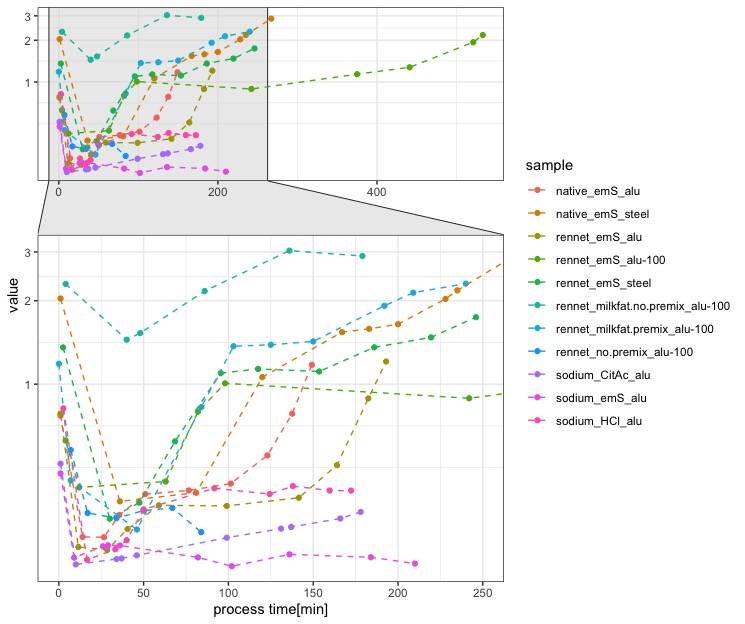
\includegraphics[width=1\linewidth]{plots/1.1_sum.rheo} \caption[Overview of measured apparent viscosities in samples during model testing]{Overview of Viscosity Development during structure-formation reaction in model processed cheeses varying either in composition (native, rennet or sodium casein[ate] with the mixture of emulsifying salts used herin [emS] or sodium caseinate with either [HCl] or citric acid [CitAc] for pH adjustment), preparation (pre-homogenisation [premix, no.premix] and pre-emulsification of fat [milkfat, oil is the default]) or processing conditions (heat-transfer i.e. free Energy [alu, steel], or shear rate i.e. mixing/aggregation rate [alu-100, alu 200/s is the default])}\label{fig:unnamed-chunk-5}
\end{figure}

\begin{figure}
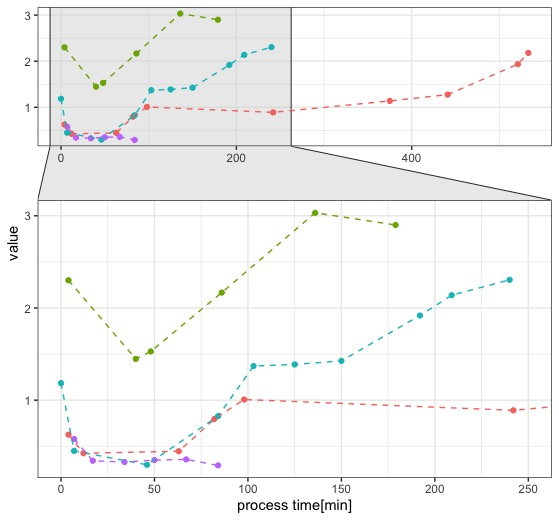
\includegraphics[width=0.75\linewidth]{plots/1.2_fatvar.rheo} \caption[Effect of premixing on the rheological profile of tested samples]{Comparison of Rheological profile during structure formation of pre-homogenised (red, blue) or non-homogenised (violet, green) samples and of pre-emulsified (green, blue) fat (in form of milkfat) or unemulsified (red, violet) fat (in form of oil). Note that the red and violet curves are identical in their composition but vary in terms of pre-homogenisation.}\label{fig:unnamed-chunk-6}
\end{figure}

Fig.xx shows the viscosity increase of the tested models that were
different in their oil composition. If the fat source was dairy cream,
structure formation took place even without an premixing step (green).
The aim of this work was, however, to investigate \emph{inter alia} the
emulsification properties and further potential aggregation of casein
coated fat globules or particles, at later stages of processing. To do
so, no pre-emulsified fat other than emulsified with caseins, should be
present. Milk fat is pre-emulsified fat, The milk fat globule is
stabilized by milkfat globule membrane proteins. Therefore, plant oil in
the form of sunflower oil was used as the dispersed phase. However,
without a pre emulsifying step which is furthered referred to herein as
premixing was included in the sample preparation. The effect of
premixing can be found in Fig.xx as well, the violet points show a
non-premixed system, the red points are the same sample, processed after
premixing at \textasciitilde8000 rpm.

\begin{figure}
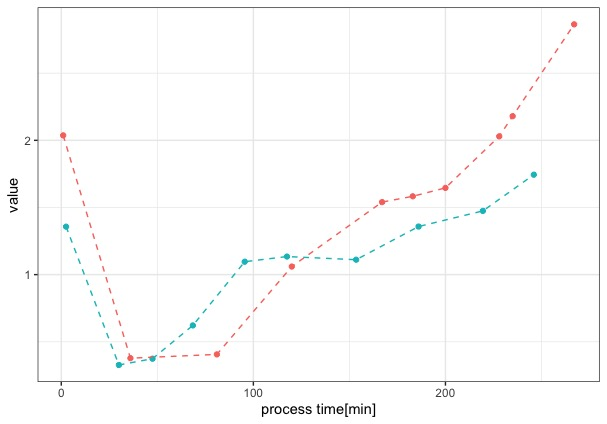
\includegraphics[width=0.75\linewidth]{plots/1.4_steel.alu.sum} \caption{Rheological Profile of samples made from native (red) or rennet (blue) casein, processed in a steel cup}\label{fig:unnamed-chunk-7}
\end{figure}

The overall rheological profile of samples made from native or rennet
casein, differs only slightly. Native casein samples show a faster
structure formation than rennet casein samples, as well as an overall
higher viscosity. This can be due to the different initial particle
sizes of the casein powders, since the rennet casein powder had a more
granular consistency, whereas the native casein powder was powdery.
@Dickinson2012 described the formation of stronger gels from
inhomogenously hydrated or dispersed samples, due to faster
bridging-flocculation of the fat particles. Bridging-flocculation was
promoted by vast amounts of unadsorbed and also in parts unhydrated
protein or casein particles. This also lead to a prefered formation of
particulate fat globules and thus, for an emulsion filled gel to the
formation of a particle gel. This is represented in Fig.xx by the faster
processing of the native casein model cheeses, since a particle gel has
a higher rigidity than an emulion filled gel.

\begin{figure}
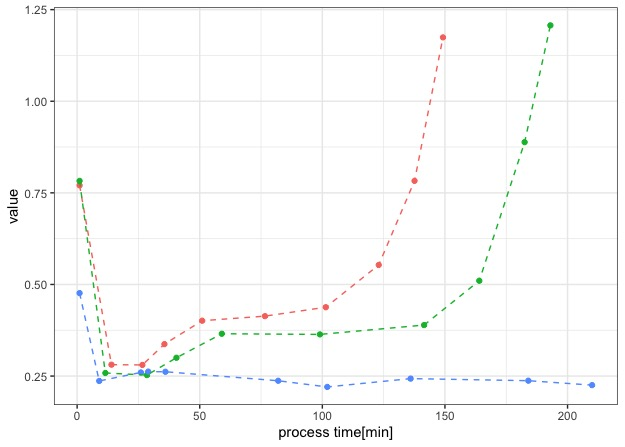
\includegraphics[width=0.75\linewidth]{plots/1.5_source.vari} \caption[Overview of viscosity, depending on the protein source]{Rheological Profile of samples made from native (red), rennet (green) or sodium (blue) caseinate,  processed with the mixture of emulsifying salts used herein in an aluminium cup. The processing conditions for these samples were set to the standard conditions for further analysis.}\label{fig:unnamed-chunk-8}
\end{figure}

When comparing Fig.xx and Fig.xx it becomes apparent, that the aluminium
cup leads to faster processing, which is due to a better heat transfer
of the aluminum and the higher porosity in the aluminium cup, which
might provoke an autocatalytic effect. Comparing the shear rates, we see
that the process speed is dependent on the shear rate, which is in
conclusion with rheological behaviour for non-Newtonian fluids, as well
as with the faster structure formation (i.e.~higher reaction rate), due
to higher probability of collision of the particles. Faster processing
by higher shear rates was also reported by @Fu2018.

The model testing led to the model composition of Table 1. For faster
sample throughput, a processing speed of 200/s in the aluminum cup was
chosen. The premixing step was made standard protocol for sample
preparation and was set to not exceed 10.000 rpm.

\newpage
\subsection{Results and discussion}

\subsubsection{Flow curves during processing of model processed cheeses}

The composition of model process cheese (Table 1) lead to a dry mater of
40 \% with protein concentrations from 15-17\% TP, depending on the
total protein content of the source material. Samples were pre-mixed
prior to processing, since it was found that without an initial
emulsification step, no stable educt (melt/sol) could be produced in the
processing cup. It should be noted that @Lenze2019 used pre-emulsified
fat (milk fat or oil + small molecule surfactants) in the process which
led to the stable educt.

\begin{figure}
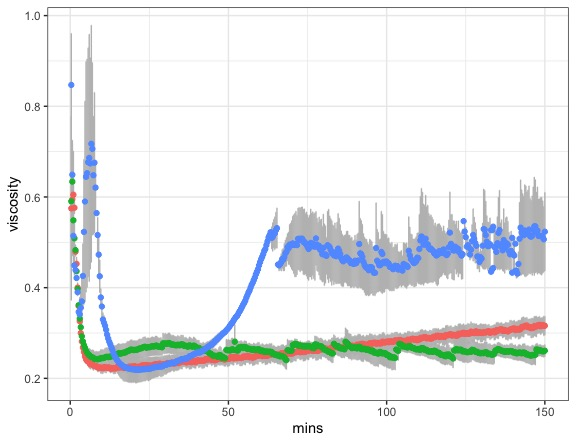
\includegraphics[width=0.75\linewidth]{plots/1.6_sodium.detail} \caption[measured apparent viscosity of models with sodium caseinate]{Detailed rheological profile of model processed cheese samples made with sodium caseinate as source material.  Variation was in the type of salt used for pH adjustment to a value of 5.88:  HCl (blue), Citric Acid (red), emulsifying salts (green).  Measurements were performed in triplicate and plotted as mean; variation in viscosity indicated as grey shade.}\label{fig:unnamed-chunk-9}
\end{figure}

Fig.xx shows the flow curves of the processed sodium samples. When
processed without melting salts but HCl as pH adjustment, we can see a
structure development up to a first plateau (blue). After that, no
further structure development could be recorded. The compared to the
other samples rather high standard deviations represent a cohesiveness
of the matrix at this point, represented by a strong tendency to pull
strings, when sampled after 150 minutes. @Vollmer2021 reported that
kappa casein fibrils in a similar model processed cheese made from
native casein were the key element for structure formation in model
processed cheeses, since their supposed building could be followed as
well as their structuring of the matrix. Kappa casein is the only casein
that is not affected by calcium, which also means that it is not
influenced by the ion exchange process that is used for the production
of sodium caseinate, as described in the next paragraph. Therefore kappa
casein is present in its more or less native state, at least from the
point of view of ionic substitutes. Hence, the detectable increase in
apparent viscosity from a level of 0.2 to \textasciitilde0.5 between 40
and 60 minutes of processing could be assigned to an adsorption of kappa
casein fibrils to the interphase, possibly as the only larger aggregate
present in the system.

In the green curve which was processed with emulsifying salts, no
structure build-up could be detected. This might be due to the little
amounts of calcium being available in the sodium caseinate samples, thus
a far lesser concentration of Calcium Ions can be released into the
serum. Sodium caseinate is generated by acid percipitation of caseins
with subsequent alkalization and final neutralization; a process that
forms single caseinates, wherein the calcium ions are to some degree
replaced with sodium ions, whereby the CCP are completely absent. This
means that the remaining calcium ions in sodium caseinate are small in
number and directly bound to phosphoserine residues. Chelation of the
calcium phosphate nano clusters from the micelle up to a value of 70\%
is reported to lead to full dissociation of the micellar structure
(@Fox2016). In @Vollmer2021a, a critical threshold value of PP of 1.2\%
is shown, to induce complete dissolution of CCP from the micelle. Hence
it can be concluded, that the threshold value for complete micelle
dissociation is reached within this study and the caseins are present in
monomeric form.

It can be suggested that the initially chelated calcium ions in samples
made from rennet or native casein are not immobile, or even inertly
bound in their chelated complexes, but could participate in processes
that lead to aggregation. This will be discussed in further detail
during this work.

\begin{figure}
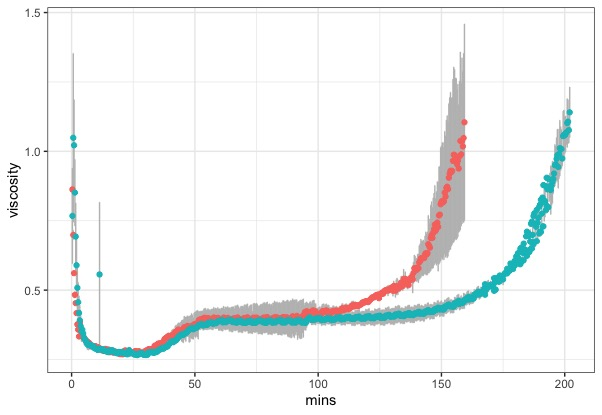
\includegraphics[width=0.75\linewidth]{plots/1.7_nat.ren.datail} \caption[Measured apparent viscosity of native and rennet casein]{Detailed rheological profile of model processed cheese samples made with native casein (red), or rennet casein (blue) as source material.  Measurements were performed in triplicate and plotted as mean; variation in viscosity indicated as grey shade.}\label{fig:unnamed-chunk-10}
\end{figure}

Native casein samples build up their structure slightly faster than
samples made from rennet casein. Also, native casein had a higher
variance in total process duration. The first stages of structure
formation up to a processing time of \textasciitilde100 minutes however,
show no difference concerning the source material. The start of the
second phase of structure formation is up to 50 minutes earlier than in
samples made from native casein. This could attributed to higher matrix
inhomogenity of the native casein samples, due to smaller particle size
of the powder. When pre-mixing the samples, it was observed that the
smaller particle size of the Native Casein showed powdered clusters. It
has been previously reported, that a higher matrix inhomogenity, like
the appearance of such powdered clusters, leads to higher gel
stabilization in emulsion filled gels due to a faster bridging
stabilization of the oil droplets (@Oliver2016, @Dickinson2012). Such a
bridging stabilzation was shown to be induced by excess unadsorbed
protein (@Semenova2010). The rennet casein premixes showed a coarser
structure, since the grain size was around 0.1 mm. Thus, the matrix
hydrates more slowly, as indicated in the slightly later starting time
of the first exponential phase.

\begin{figure}
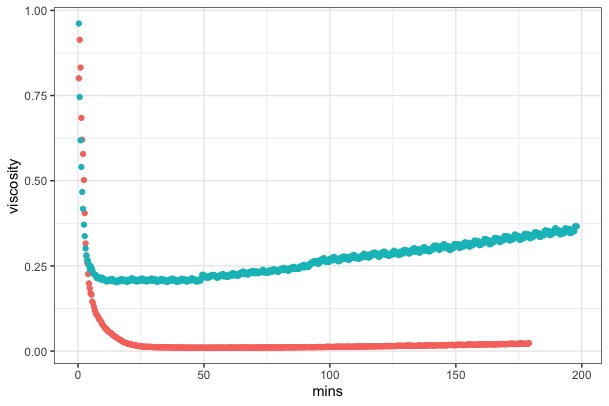
\includegraphics[width=0.6\linewidth]{plots/1.8_control} \caption[Apparent viscosity of sodium caseinate and native casein controls]{Rheological profile of control samples w/o any addition of salts: native casein (red) and sodium caseinate (blue)}\label{fig:unnamed-chunk-11}
\end{figure}

Controls show that native casein without any addition of emulsifying
salts at native pH (6.57) shows a slow, if any, structure formation
after about 125 min of processing. This is probably due to the slight
heat induced dissociation of the casein micelle, and/or a possible
re-aggregation of released caseins therefrom. Sodium caseinate shows a
higher level of viscosity after melting (0.2) than the native control,
which was measured at \textasciitilde.03. The native control did not
produce a stable emulsion or gel evenly during heat-processing; a watery
opaque liquid with free fat was apparent next to clumped,
i.e.~amorphously aggregated structure. Samples from sodium caseinate
without the addition of salts did form a stable premix and also showed
structure formation.

The comparison of the controls shows, that when processed without salt
addition at native pH an overall increase of 0.11 a.u. in viscosity
takes place, similar to the increase measured in models with sodium
caseinate and citric acid. Slight step-wise increases in viscosity can
be seen at 50 min and at 100 min. Those were also the process times,
where exponential increases in viscosity were detected in the model
samples. It can be concluded, thet the phosphate and citrate salts,
maybe also in combination with their respective sodium cations are
responsible for the abundance of a detectable viscosity increase in
samples from sodium caseinate made with emulsifying salts.

\subsubsection{pH values post-processing}

\begin{figure}
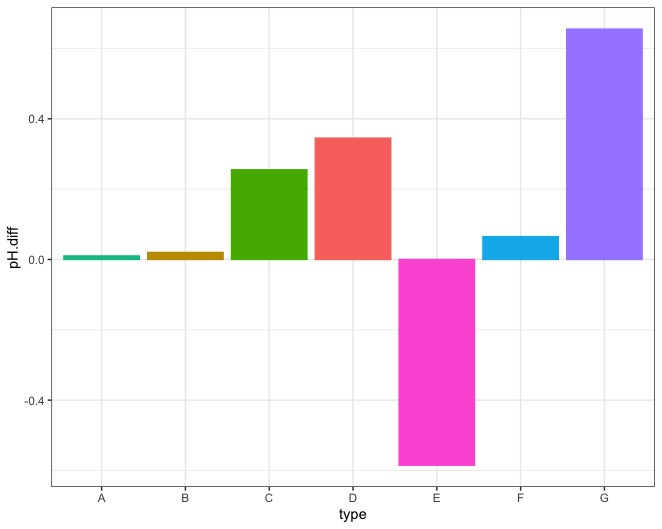
\includegraphics[width=0.6\linewidth]{plots/1.9_pH} \caption[Difference in pH value of tested samples after processing]{Difference in starting pH of the sample premix and pH of the sample product after processing:  (A) sodium caseinate w/o emulsifying salts; (B) native casein w/o emulsifying salts;  (C) rennet casein with emulsifying salts; (D) native casein with emulsifying salts; (E) sodium caseinate with HCl; (F) sodium caseinate with citric acid; (G) sodium caseinate with emulsifying salts}\label{fig:unnamed-chunk-12}
\end{figure}

The pH for all samples was set to 5.88 +/- 0.02, prior to processing.
Samples from rennet casein and native casein showed an increase in pH
over the course of the reaction (up to 6.17), samples from sodium
caseinate showed a slight increase in pH for samples made with citric
acid but no additional calcium chelators up to 5.86 +/- 0.01. The
strongest increase in pH was apparent for samples made from sodium
caseinate with emulsifying salts: pH of the processed sample rose to
6.48 +/- 0.02. Only the samples made of sodium caseinate and HCl
(i.e.~without any Calcium chelating agents) showed a decrease in pH to
5.22 +/- 0.01. The decrease might be due to over aciding as the matrix
was strongly coagulated already during premixing, so the initial pH
might have been indeed at a lower level to begin with, and expressed
itself only after melting. These samples also showed a structure
formation up to the first exponential and second log phase of
processing. Due to the low pH, it could be also possible that this is
not an effect induced by kappa casein (-fibrils), but due to beta casein
being close to its IEP (5.20) and therefore emulsifying the fat phase.
We can see that the emulsifying salts otherwise generally increase the
pH of the samples and thus change the charge in the casein molecules
more negatively. The strong pH increase detected in sodium caseinate
samples processed with emulsifying salts could be due to certain degrees
of dephosphorylation of the calcium sensitive caseinates (alphaS1,
alphaS2 and beta casein). Since the hydroxy group of the corresponding
Serin residue is a far weaker acid than the respective phosphate group,
the pH of a casein containing matrix will increase with ongoing
de-phosphorylation of the caseines.

Buffering the pH at the desired value is crucial for the properties of
the final product, a lower processing pH (5.2 - 5.6) resulted in more
coarse and particulate gels, whereas a pH value of 5.8 - 6.2 gave creamy
products (@Barth2017). It is apparent, that the pH value in the model
samples from native and rennet casein was buffered in the desired range,
whereas the samples made from sodium caseinate couldn't be buffered at
the target level.

\subsubsection{Occurence of a third log phase and the fitting of a model flow curve}

In another embodiment of the experimental set-up, rennet casein samples
were processed in a steel cup, using the same temperature and speed
settings. To the authors surprise, longer processing times were needed
and the rheological profile appeared to be different than the samples
processed in the aluminum cup. In total, the steel cup lead to
\textasciitilde30\% longer processing times. However, in relation to the
respective full process times, the time needed for the first and second
exponential phases to start, displayed the same ratio. In Fig.xx the
appearance of another plateau phase during the second exponential phase
is visible between 12.000 and 15.000 seconds of processing. This plateau
phase was also seen in the flow curves of the samples analyzed by
@Vollmer2021. Since the samples in @Vollmer2021 were processed at half
the processing speed, the occurence of the additional plateau phase
seems to display an intermediate halt of structure formation. It is
reported that the occurence of large fibrillar structures are very
electron dense, i.e.~high in protein, next to areas, where a low
electron density is apparent. Before the display of the plateau phase,
the casein fibrils appear in bundles, during the plateau phase, these
bundles get broken down, which seems a reasonable explanation for this
effect. Also, it is to be expected, that this part of the second log
phase only displays itself in the set-up with an aluminum cup, due to
the different physical properties of steel and aluminum.

\begin{figure}
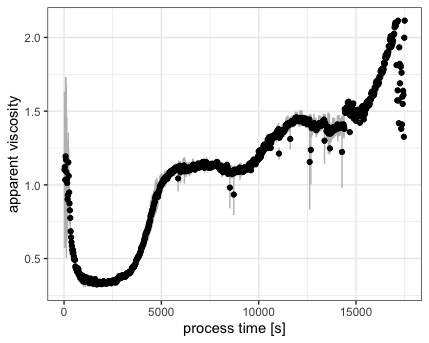
\includegraphics[width=0.5\linewidth]{plots/6.1_visco.mean.steel} \caption[Structure formation in a steel cup]{Plotted mean values of the measured apparent viscosity of model processed cheese samples produced from rennet casein prepared in a steel cup: a third lag phase, which represents an intermediate stabilization at an apparent viscosity level during the second exponential phase of structure formation, was observed.}\label{fig:unnamed-chunk-13}
\end{figure}

Firstly, aluminum has an \textasciitilde5 times higher heat transfer
capacity than steel. Also, the aluminium cup displayed a higher friction
of the samples due to adherence of the matrix to the walls of the cup.
This puts a higher amount of shear stress on the sample, induced by the
sample itself. Higher shear led to faster processing in general, as it
was shown during model development. It is also possible, that an
autocatalytic effect took place in the aluminum cup. The addition of
pre-processed sample to a new matrix was shown to induce a rapid
increase in structure development (@Fu2018, @Cernikova2018a,
@Lenze2019). It is thinkable, that this effect took also place here to a
certain degree, but in-situ by seed formation in pores or cracks of the
aluminum cup.

In various other studies, model process cheese matrices similar and
compareable to this system were processed by differently shaped means.
The unity of all means of processing, either kneading type shearing
using a Farinograph as in the works of @Noronha2008c, or processing at
high speed using a rapid viscometer as in @Fu2018, a step-wise structure
formation is reported. The different structure formation curves that
showed a step-wise or two phased process as indicated by exponential
increase in apparent viscosity were used to fit a general rheological
profile for the model processed cheese, also for the use in later
correlation analysis. The flow-curves of native as well as rennet casein
were used for the modellation, since it was shown in @Roeck2010 and also
in this study, that the two protein species displayed no large
differences in apparent viscosity.

In order to get the pronounced two step process but also a dynamic lag
phase represented in a fitted viscosity model, not the model with the
best fit was chosen, but with a good empirical estimation under
consideration of the R\^{}2 of the fit. By including the variance of a
later or earlier occuring second exponential phase, i.e.~the effect of
matrix inhomogenity, either due to different fat globule size or powder
particle size, which occured during the pre-mixing step, could be
included in the model. The plotted mean curves with their respective
variance can be found in the supplementary material. To also include the
intermediate stabilization described earlier, the curves from the steel
cup were also included in the fit. The flow curve was fitted using a
generalized additive model. Such ``gam'' models with integrated
smoothness estimation are impelemented within the R programming
language, which was used to prepare this thesis. The `gam' function for
basic model fitting takes into account any quadratically penalized
general linear model. This means that the regression of every data point
or linear sets therefrom are considered within the model. To prevent
from over-fitting, the degree of smoothness of model terms is estimated
as part of fitting. In more detail, a generalized additive model of the
form

\emph{g(mu\_i) = b0 + b1x1i + b2x2i + f(x3i) + f2(x4i, x5i)}

wherein the response variable, in our example the viscosity, is
represented as an expectation \emph{mu\_i} withing a link function
\emph{g()}. The general additive model (``gam'') of this formula would
then be

\emph{y \textasciitilde{} x1 + x2 + s(x3) + s(x4,x5)}.

Per definition of ``gam'' within R, a maximum smoothing term is applied
and the fitted

\emph{y(x) = g(s(x))}

resulted in an R\^{}2 = 0.71. As it is the case for many built-in
numeric operations in R, the algorithm for the general additive model
has an implemented, nested two-side ANOVA test. The fitted values are
displayed in Fig.xx.

\begin{figure}
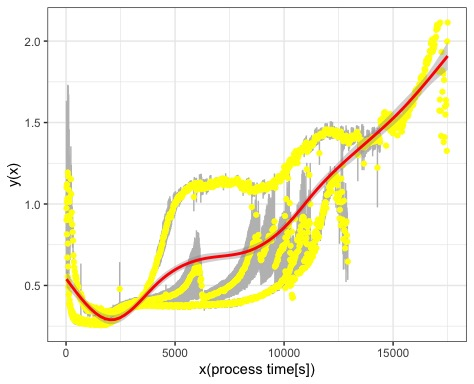
\includegraphics[width=0.75\linewidth]{plots/6.11_visco.fit.high.smooth} \caption[fitted model flow curve]{Fitted residuals from the function from the general additive model, applied with internal cubic spline smoothing term; yellow is the data, grey is thes standard deviation from the data and the red line represents the fitted values.}\label{fig:unnamed-chunk-14}
\end{figure}

\subsection{Summary and outlook}

In this section, a multi-step structure formation for samples made from
rennet and native casein could be reported. A ``one-step'' structure
formation was found in samples made from sodium caseinate processed with
HCl (to adjust the educt pH to the target value of 5.88) but no further
use of buffering salts or agents. Thsi type of structure formation was
attributed to soluble beta casein adsorbing to the o/w interphase and
thereby decreasing the overall elasicity of the system. The samples made
from rennet casein and native casein, displayed similar behaviour,
variances were attributed to varying matrix inhomogenity. The targeted
step-wise structure formation as it was displayed in @Lenze2019 could be
reproduced with an improved model processed ceese system. Furthermore
the indifference of native or rennet casein to be used to form the
targeted structure could be confirmed.

Interesting here as well was the behaviour of sodium caseinate in
relation to the degree of calcium deprivation. The rest of calcium ions
in sodium caseinate is directly bound to phosphoserine residues. When
processed without melting salts, we could see a structure development up
to the first plateau. After that, no further structure development could
be recorded. Combining the models suggests that the initially chelated
calcium ions in samples made from native or rennet casein are not
immobile or inert in the system within their chelated complex, but can -
and will after time- initiate a second structure formation phase, i.e.~a
second growth phase. Samples made from sodium caseinate, that were still
calcium deprived but had no pH buffering (i.e.~the sodium caseinate
model with HCl) showed an increase in viscosity. Thus the mobility of
the caseins to form self-assemblies like in the HCl model as well as the
inhibition of structure formation through the lack of Calcium ions could
be shown in this section.

For samples made from sodium caseinate, there seems to be no inner force
or linking agent to form a secondary structure as seen in samples made
from initially micellar (native or rennet) caseins. This is surprising
since the levels of PP to induce complete dissociation of the micelle by
chelation of CCP were above the reported threshold in similar models
(@Vollmer2021a). Therefore, sodium and native models should present
caseins in monomeric structure after melting. The caseins even have
suspectedly the same ionic subsitute, since sodium salts were used. It
can be suggested that the presence of large amounts of previously
colloidal calcium is forcing the proteins to either deplete from the
solved calcium ion or readily bind to it. @Depletion

One aim of this study was to find. models with high similarity in
composition (ionic environment and strength) but with very different
struture formation properties. Native and Rennet Casein samples showed
no significant difference in the overall shape of the structure
formation, only the start of second exponential phase showed variance.
This effect can be attributed to a differing matrix homogeneity due to
differing powder-particle-sizes.

Since calcium is long known to be the factor stabilizing caseinate based
emulsions (@Dickinson1998), the null model for the creaming process,
i.e.~the model system that had similar composition but showed no
structure formation could be identified. This model was the sodium
caseinate system, processed with emulsifying salts. As expected, calcium
deprived emulsion gels didn't show structure formation. Therefore the
two models that were investigated in their respective composition (see
section 4) were chosen to be native casein and sodium caseinate,
prepared with oil in a premixing step and processed with emulsifying
salts.

The findings herein are in conclusion with findings of other works
concerning the creaming reaction, but especially in the context of this
work and the connected studies performed by @Lenze2019, @Vollmer2021 and
@Vollmer2021a. The modellation of a characteristic flow curve was
performed and will be used later within correlation analysis of the
experimental data. The modelled flow curve resembled the shape of the
flow curve presented in @Vollmer2021.

\end{document}
